\let\negmedspace\undefined
\let\negthickspace\undefined
\documentclass[journal]{IEEEtran}


\setlength{\headheight}{1cm} % Set the height of the header box
\setlength{\headsep}{0mm}     % Set the distance between the header box and the top of the text
 \usepackage[a4paper,margin=10mm, onecolumn]{geometry}
\usepackage{gvv-book}
\usepackage{gvv}
\usepackage{cite}
\usepackage{amsmath,amssymb,amsfonts,amsthm}
\usepackage{algorithmic}
\usepackage{graphicx}
\usepackage{textcomp}
\usepackage{xcolor}
\usepackage{txfonts}
\usepackage{listings}
\usepackage{enumitem}
\usepackage{mathtools}

\usepackage{gensymb}
\usepackage{comment}
\usepackage[breaklinks=true]{hyperref}
\usepackage{tkz-euclide} 
\usepackage{listings}                                       
\def\inputGnumericTable{}                                
\usepackage[latin1]{inputenc}                                
\usepackage{color}                                            
\usepackage{array}                                            
\usepackage{longtable}                                       
\usepackage{calc}                                             
\usepackage{multirow}                                         
\usepackage{hhline}                                           
\usepackage{ifthen}                                           
\usepackage{lscape}
\usepackage{circuitikz}
\tikzstyle{block} = [rectangle, draw, fill=blue!20, 
    text width=4em, text centered, rounded corners, minimum height=3em]
\tikzstyle{sum} = [draw, fill=blue!10, circle, minimum size=1cm, node distance=1.5cm]
\tikzstyle{input} = [coordinate]
\tikzstyle{output} = [coordinate]

\begin{document}

\bibliographystyle{IEEEtran}
\vspace{3cm}

\title{1.3.4}
\author{AI25BTECH11025-R Nikhil}
 \maketitle
% \newpage
% \bigskip
{\let\newpage\relax\maketitle}

\renewcommand{\thefigure}{\theenumi}
\renewcommand{\thetable}{\theenumi}
\setlength{\intextsep}{10pt} % Space between text and floats


\numberwithin{equation}{enumi}
\numberwithin{figure}{enumi}
\renewcommand{\thetable}{\theenumi}


\section*{1.3.4}
If $ A(1, 3), B(-1, 2), C(2, 5) $ and $ D(x, 4) $ are the vertices of a parallelogram  ABCD , then the value of $x$ is \underline{\hspace{2cm}}(10, 2012)

\vspace{1em}
\textbf{Solution:}

In a parallelogram, the opposite sides are equal. Therefore, the length of side AC equals to the length of side BD:

\begin{align}
\vec{C} - \vec{A} = \vec{D} - \vec{B} \\
\vec{D} = \vec{B} + \vec{C} - \vec{A}
\end{align}


Substituting the coordinates:
\begin{align}
\myvec{ x \\ 4 } = \myvec{ -1 \\ 2 } + \myvec{ 2 \\ 5 } - \myvec{ 1 \\ 3 } \\
                 = \myvec{ -1 + 2 - 1 \\ 2 + 5 - 3 } \\
                 = \myvec{ 0 \\ 4 }
\end{align}

This gives us the equations: 

\begin{align}
    x=0  \\
    4=4
\end{align}

\textbf{Answer:}  
\textbf{x=0}

\begin{figure}[h!]
    \centering
    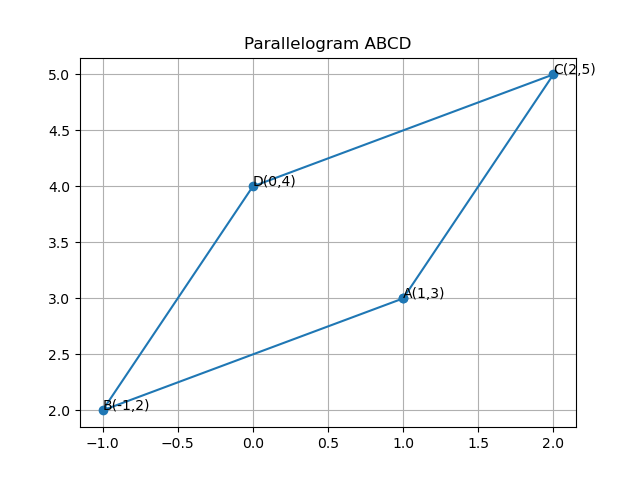
\includegraphics[height=0.5\textheight, keepaspectratio]{figs/plotc.png}
    \label{figure_1}
\end{figure}

\end{document}
